
\subsection{}
\begin{definition}
    Economics is a social science that studies how we allocate limited resources
    to satisfy unlimited wants.
\end{definition}
\begin{definition}
    Social science is the study of people.
\end{definition}
Is the allocation of resources fair? just? efficient?
By resources we mean:
\begin{itemize}
    \item Land (T)
    \item Labour (L)
    \item Capital (K) 
\end{itemize}
Note: Money is not a resource, it is a means of making exchange easier.
With Land, Labour or Capital you could make use of them on a island alone.

These resources are limited or scarce but \textbf{our wants are unlimited}. Even billionaires give away their money for their wants.
Scarcity $\rightarrow$ Choice.
\newpage
\begin{figure}[h!]
    \begin{minipage}{\textwidth}
        \centering
        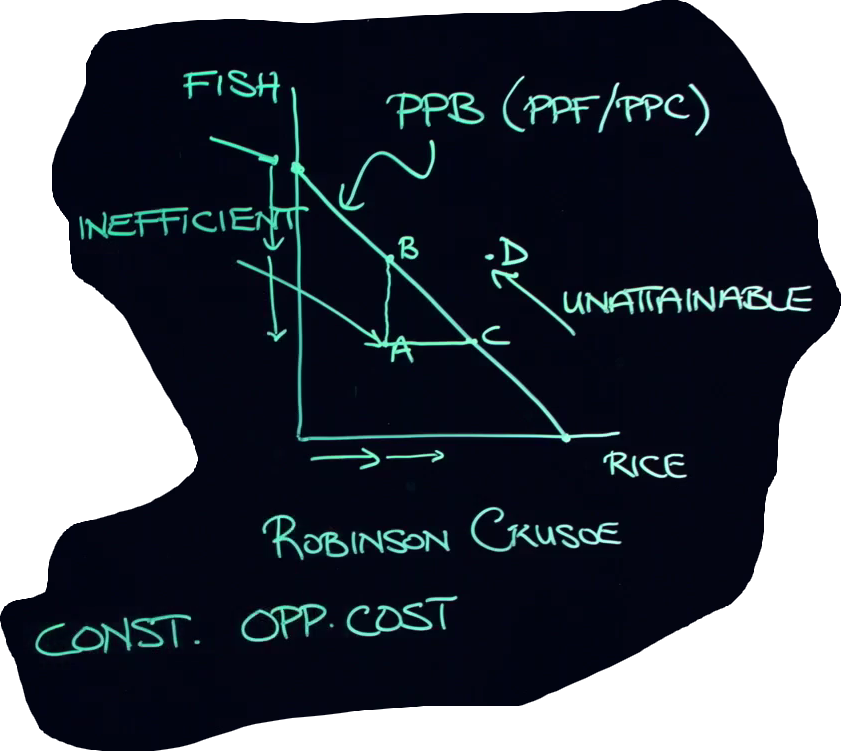
\includegraphics[width=0.5\textwidth]{RobinsonConstant.png}
        \caption[Constant Opportunity Cost]{Robinson Crusoe\footnote[1]{Story of a life of comfort to a solitary existence on a deserted island}'s Constant Opportunity Cost}
    \end{minipage}
\end{figure}
\begin{center}
\end{center}
Naturally we try to equalize the values of rice and fish (EQUITY).
If we used all of Crusoe's resources we would get a linear line (PPB/PPF/PPC meaning Production Possibility). Say that point A is below the line. This means it is potential with his resources but we say it is \textbf{inefficient}.
Same with point B and C but they maximize his resources. Point D is above the line and is \textbf{unattainable}, meaning he cannot achieve it.

\begin{definition}
    Opportunity Cost is the value of the next best alternative forgone.
    \begin{example}
    If Crusoe has maximized his use of resources, to acquire more rice, Crusoe must give up some fish.
    The cost is constant in this example.
    \end{example}
    Note: In real life, a constant opportunity cost is generally not realistic.
\end{definition}
\newpage
Imagine Crusoe's opportunity cost is no longer constant but increasing.
The graph of his resources would be a slope.\\
\begin{figure}[h!]
    \centering
    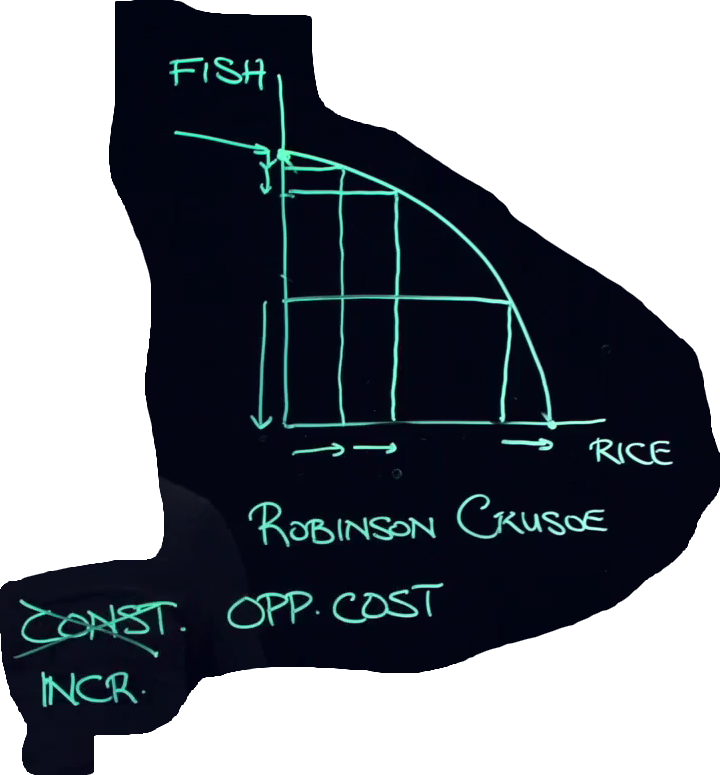
\includegraphics[width=0.5\textwidth]{RobinsonIncreasing.png}
    \caption{Robinson Crusoe's Increasing Opportunity Cost}
\end{figure}
Crusoe is able to give up the inefficent methods of obtaining fish/rice for the other initially.
To obtain more and more of the other, he must give up more and more of the other. This is the law of increasing opportunity cost.
